\subsubsection{Schaltungen}
\label{sec:schaltungen}

Die Schaltungen wurden von Kevin Cornelius entworfen.
Es wurden lediglich sehr einfache Schaltungen verwendet.
\begin{enumerate}
	\item Die wichtigste Schaltung stellt hier die Infrarot-Diodenschaltung dar. Diese besteht aus der Infrarot-Diode (LD-274-3, Sendefrequenz 56kHz) inklusive Vorwiderstand und einem Verstärkerteil, welcher aus einem Widerstand und einem Transistor (T547C) besteht.\\
	\begin{figure}[h]
		\centering
		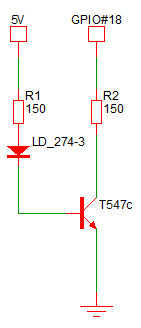
\includegraphics[width=0.2 \textwidth]{./040-komponenten/010-hardware/Diodenschaltung.png}
		\caption{Die Dioden-Schaltung}
		\label{fig:Bild2Hardware}
	\end{figure}\\
	Mit dieser in \cref{fig:Bild2Hardware} zu sehenden Schaltung schafft man es, das Signal so zu verstärken, dass man eine Reichweite von ca. fünf Meter hat. Dies ist für ein Indoor-Lasertag ausreichend.
	\item Die zweite in \cref{fig:Bild3Hardware} dargestellte Schaltung ist zum Auslösen des „Taggers“. Sie enthält nur einen Vorwiderstand und einen Push-Button. \\
	\begin{figure}[h]
		\centering
		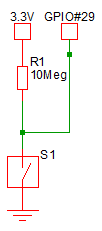
\includegraphics[width=0.2 \textwidth]{./040-komponenten/010-hardware/Button.png}
		\caption{Die Button-Schaltung}
		\label{fig:Bild3Hardware}
	\end{figure}\\
	Wenn der Button gedrückt wird, wird der Stromkreis geschlossen und der Tagger schießt.
	\item Die dritte Schaltung, die in \cref{fig:Bild4Hardware} gezeigt wird, ist die der Anzeige-LEDs. Es sind drei in unterschiedlichen Farben (grün, gelb und rot), welche jeweils an einem einzelnen GPIO-Pin liegen. Außerdem wurde ein Vorwiderstand verwendet.\\
	\begin{figure}[h]
		\centering
		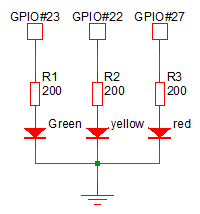
\includegraphics[width=0.3 \textwidth]{./040-komponenten/010-hardware/LEDschaltung.png}
		\caption{Die LED-Schaltung}
		\label{fig:Bild4Hardware}
	\end{figure}\\
	Die LEDs können einzeln angesteuert werden und so verschiedene Spielzustände anzeigen. Die Funktion wird genauer im \cref{sec:leds} beschrieben.
	\item Der Empfänger ist ein TSOP31256 und an Stromversorgung, Erdung und GPIO-Pin angeschlossen.\\
	Er empfängt auf einer Frequenz von 56kHz, welche dazu führt, dass man eine höhere Reichweite erreicht und weniger Signalstörungen hat.

\end{enumerate}
